\subsection{Role of Depth, Width and Skip Connections}\label{sec:mem}
We now look at a simple memorisation task, wherein, given a dataset of just values $(y_s)_{s=1}^n\in  \R$, the aim is to accept $s\in[n]$ as input and recall $\hat{y}_{\Theta}(s)\approx y_s$. The loss of the memorisation task is defined as $L_{\Theta}=\frac{1}{2}\sum_{s=1}^n (\hat{y}_{\Theta}(s)-y_s)^2$. For this task, we compare two architectures namely (i) residual DGN (ResDGN) of $(b+2)$ blocks, where each block is a fully connected DGN of width `$w$', depth $\dblock$ (total depth $d=(b+2)\dblock$) and (ii) fully-connected DGN (FC-DGN) of width`$w$' and depth $d=(b+2)\dblock$. In both these DGNs, there is no gating network, however, for each index $s\in[n]$, the gating values $G_{s}(i,l),\forall l\in[d-1], i\in[w] $ are randomly set to be $0$ or $1$ (with equal probability) and kept fixed throughout training. Further, in both these DGNs, the input is fixed as $1\in\R$ and the weights of the value network are sampled as per \Cref{assmp:main} with $\sigma=\frac{2}{w}$. 
For this choice of the gates it follows that $\E{\frac{H^{\text{lyr}}(s,s)}{w}}=\frac{1}{2}$, $\E{\frac{H^{\text{lyr}}(s,s')}{w}}=\frac{1}{4},\,\forall s\neq s'$. Since the input is $1\in\R$, the input Gram matrix $\Sigma$ is a $n\times n$ matrix with all entries equal to $1$. Putting all this together, it follows that $\E{K^{\text{fc}}_0}(s,s)=d$,  $\E{K^{\text{res}}_0}(s,s)=\sum_{\J\in 2^{[b]}}  \bres^{\J}$, $\E{K^{\text{fc}}_0}(s,s')=d\cdot\left(\frac{1}2\right)^{d-1}$ and $\E{K^{\text{res}}_0}(s,s')=\sum_{\J\in 2^{[b]}}  \bres^{\J}\left(\frac{1}2\right)^{(|J|+2)\dblock-1}$.

Here, a set of values $(y_s)_{s=1}^n\in  \R$ is given, and the memorisation network (with weights $\Theta\in\R^{\dnet}$) accepts $s\in[n]$ as its input and produces $\hat{y}_{\Theta}(s)\approx y_s$ as its output. The loss of the memorisation network is defined as $L_{\Theta}=\frac{1}{2}\sum_{s=1}^n (\hat{y}_{\Theta}(s)-y_s)^2$.  The input to the memorisation network is fixed as $1\in\R$, and for each index $s\in[n]$, the gating values $G_{s}(i,l),\forall l\in[d-1], i\in[w] $ are randomly set to be $0$ or $1$ (with equal probability) and kept fixed throughout training. Thus, there is a separate random sub-network to memorise each $y_s\in\R$. 
%\FloatBarrier
\begin{table}%[h]
\centering
\begin{tabular}{| l |  l  |}\hline
Layer&  Memorisation Network\\\hline
Input  &$z_{\Theta}(0)=1$ \\
Pre-Activation & $q_{s,\Theta}(l)=\sum_{j}\Theta(i,j,l)\cdot z_{s,\Theta}(j,l-1)$\\
Hidden & $z_{s,\Theta}(i,l)=q_{s,\Theta}(i,l)\cdot G_{s}(i,l)$ \\
Final  Output & $\hat{y}_{\Theta}(s)=\sum_{j} \Theta(1,j,d) \cdot z_{s,\Theta}(j,d-1)$\\\hline
\end{tabular}
\caption{ Memorisation Network.}
\label{tb:dgnmemo}
\end{table}
\textbf{Spectrum of NTK:} For this network 
The input Gram matrix $\Sigma$ is a $n\times n$ matrix with all entries equal to $1$ and its rank is equal to 1, and hence $H_0=\Lambda_0$. We can now calculate the properties of $\Lambda_0$. It is easy to check that $\mathbb{E}_{\mu}\left[\Lambda_0(s,s)\right]=(\mu w)^{(d-1)},\forall s\in[n]$ and $\mathbb{E}_{\mu}\left[\Lambda_0(s,s')\right]=(\mu^2 w)^{(d-1)},\forall s,s'\in[n]$.  For $\sigma=\sqrt{\frac{1}{\mu w}}$, and $\mathbb{E}_{\mu}\left[K_0(s,s)/d\right]=1$, and $\mathbb{E}_{\mu}\left[K_0(s,s')/d\right]=\mu^{(d-1)}$. 
\begin{figure}
\centering
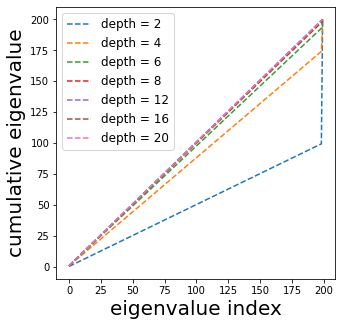
\includegraphics[scale=0.3]{figs/dgn-fra-ecdf-ideal-small.png}
\caption{Ideal spectrum of $\E{K_0}/d$ for a memorisation network for $n=200$.}
\label{fig:ideal-spectrum}
\end{figure}


\textbf{Why increasing depth till a point helps ?} 
We have:
%\comment{
\begin{align}\label{eq:mat}
\frac{\E{K_0}}{d}=\left[\begin{matrix}
1 &\mu^{d-1} &\ldots &\mu^{d-1} &\ldots\\ 
\ldots &1 &\ldots &\mu^{d-1} &\ldots\\ 
\ldots &\mu^{d-1} &\ldots &1 &\ldots \\
\ldots &\mu^{d-1} &\ldots &\mu^{d-1} &1\\ 
\end{matrix}\right]
\end{align}
%}
i.e., all the diagonal entries are $1$ and non-diagonal entries are $\mu^{d-1}$. Now, let $\rho_i\geq 0,i \in [n]$ be the eigenvalues of $\frac{\E{K_0}}{d}$, and let $\rho_{\max}$ and $\rho_{\min}$ be the largest and smallest eigenvalues.  One can easily show that $\rho_{\max}=1+(n-1)\mu^{d-1}$ and corresponds to the eigenvector with all entries as $1$, and $\rho_{\min}=(1-\mu^{d-1})$ repeats $(n-1)$ times,  which corresponds to eigenvectors given by $[0, 0, \ldots, \underbrace{1, -1}_{\text{$i$ and $i+1$}}, 0,0,\ldots, 0]^\top \in \R^n$ for $i=1,\ldots,n-1$. Note that as $d\ra\infty$, $\rho_{\max},\rho_{\min}\ra 1$.

\textbf{Why increasing depth beyond a point hurts?} 
As the depth increases the variance of the entries $K_0(s,s')$ deviates from its expected value $\E{K_0(s,s')}$. Thus the structure of the Gram matrix degrades from \eqref{eq:mat}, leading to smaller eigenvalues.
%\FloatBarrier
\begin{figure}
\resizebox{\textwidth}{!}{
\begin{tabular}{cccc}
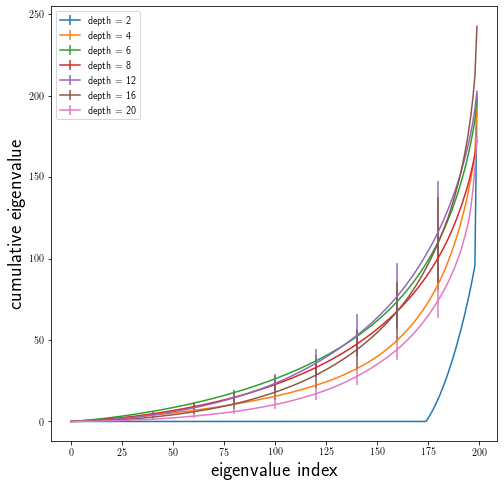
\includegraphics[scale=0.5]{figs/dgn-fra-ecdfbyd-w25.png}
&
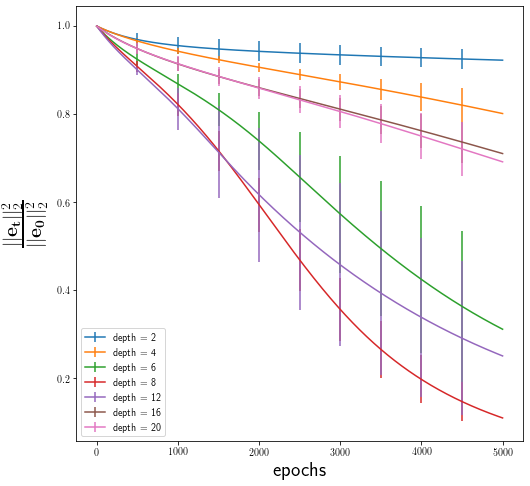
\includegraphics[scale=0.5]{figs/dgn-fra-conv-w25.png}
&
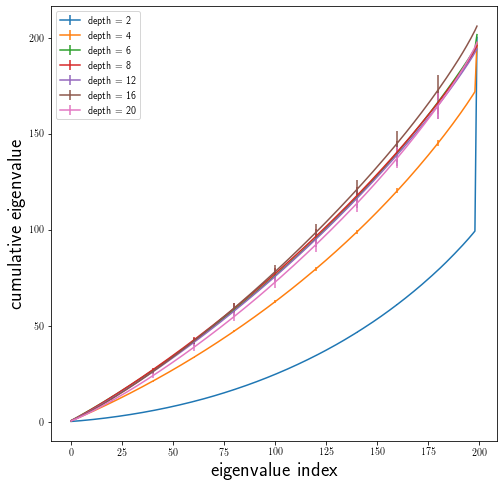
\includegraphics[scale=0.5]{figs/dgn-fra-ecdfbyd-w500.png}
&
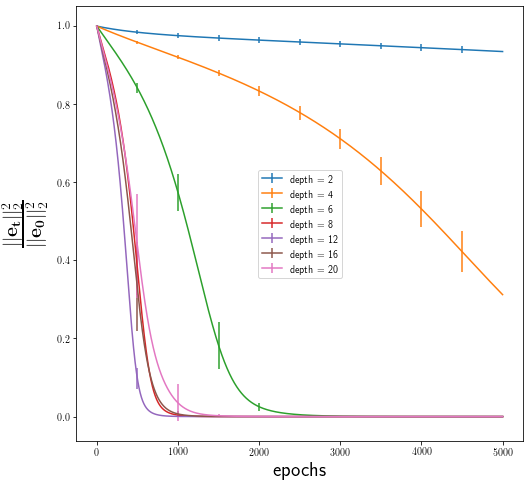
\includegraphics[scale=0.5]{figs/dgn-fra-conv-w500.png}
\end{tabular}
}
\caption{Shows the plots for the memorisation network with $\mu=\frac{1}{2}$ and $\sigma=\sqrt{\frac{2}{w}}$. The number of points to be memorised is $n=200$. The left most plot shows the e.c.d.f for $w=25$ and the second plot from the left shows the error dynamics during training for $w=25$. The second plot from the right shows the e.c.d.f for $w=500$ and the right most plot shows the error dynamics during training for $w=500$. All plots are averaged over $10$ runs.}
\label{fig:dgn-frg-gram-ecdf}
\end{figure}

\textbf{Experiment:} We set $n=100$, and $y_s\sim\text{Uniform}[-1,1]$. We look at the cumulative eigenvalue (e.c.d.f) obtained by first sorting the eigenvalues in ascending order then looking at their cumulative sum. The ideal behaviour (\Cref{fig:ideal-spectrum}) as predicted from theory is that for indices $k\in[n-1]$, the e.c.d.f should increase at a linear rate, i.e., the cumulative sum of the first $k$ indices is equal to $k(1-\mu^{d-1})$, and the difference between the last two indices is $1+(n-1)\mu^{d-1}$. In \Cref{fig:dgn-frg-gram-ecdf}, we plot the actual e.c.d.f for various depths $d=2,4,6,8,12,16,20$ and $w=25,500$ (first and third plots from the left in \Cref{fig:dgn-frg-gram-ecdf}). 

